\documentclass[11pt, oneside]{article}
\usepackage[letterpaper, margin=2cm]{geometry}
\usepackage{MATH566}
%\usepackage{sagetex}

\begin{document}
\noindent \textbf{\Large{Caleb Logemann \\
MATH 566 Discrete Optimization\\
Midterm I
}}

%\lstinputlisting[language=Sage]{03_2.sage}
\begin{enumerate}
  \item % #1 Done
    Suppose you are making a schedule for an airport.
    There are $n$ arriving flights.
    Every airplane $j$ has a possible time arrival  in interval $[a_j,b_j]$
    (plane can fly faster or slower). 
    Determine the actual arrival schedule for each airplane such that the
    smallest gap between consecutive flights is maximized
    and for all $j$, airplane $j$ arrives before $j+1$.
    Formulate a linear program that solves the problem.

    \emph{
      (Example: Suppose there are three airplanes. They have arrival intervals $[1,5],[2,7],[6,7]$.
      Then we can assign arrival times to the airplanes, for example $2,4.5,6.2$. The smallest
      gap in this schedule is $1.7$ between the second and third airplane. The number $1.7$
      is the number we want to maximize. Notice that we do not allow schedule $4,2,7$, where the first
      airplane arrives AFTER the second one although the it would be feasible with respect to $[a_i,b_i]$s
      (it is easier to solve if the order is fixed).)
    }

    First I will define a new set of variables, $t_j$ for $1 \le j \le n$, to
    be the time that plane $j$ arrives at the airport.
    Clearly we must have the constraints
    \begin{align*}
      t_j \ge a_j \\
      t_j \le b_j
    \end{align*}
    for all $j$, such  that $1 \le j \le n$.
    These constraints force each plane to arrive inside of the allowed interval
    $\br{a_j, b_j}$.
    Also if the order that the planes arrive is to be enforced, the constraints
    \[
      t_{j+1} - t_{j} \ge 0
    \]
    are required for $1 \le j \le n-1$.
    Lastly we need to set the objective function for this linear program.
    Our objective function needs to maximize the smallest time gap
    $t_{j+1} - t_j$ or in other words
    $\max* \min*_{1 \le j \le n-1}\p{t_{j+1} - t_j}$.
    I am going to create another variable $m$ to be this minimum value, that is
    \[
      m = \min*_{1 \le j \le n-1}\p{t_{j+1} - t_j}
    \]
    In this case the objective function just becomes $\max* m$.
    However we need constraints to insure that $m$ does in fact equal the
    minimum value.
    I will use the following constraints
    \[
      m \le t_{j+1} - t_j
    \]
    for all $j$ such that $1 \le j \le n-1$.
    These constraints guarantee that
    \[
      m \le \min*_{1 \le j \le n-1}\p{t_{j+1} - t_j}.
    \]
    With the addition of the objective function maximizing $m$, we will achieve
    equality.
    Therefore the entire linear program that solves this problem is
    \[
      (P) =
      \begin{cases}
        \text{maximiz}    & m \\
        \text{subject to} & t_j \ge a_j         \quad 1 \le j \le n \\
                          & t_j \le b_j         \quad 1 \le j \le n \\
                          & t_{j+1} - t_j \ge 0 \quad 1 \le j \le n-1 \\
                          & m \le t_{j+1} - t_j \quad 1 \le j \le n-1 \\
      \end{cases}
    \]
    Note that there is no minimum value of $m$ and we aren't enforcing
    nonnegativity to the variables $t_j$ as the intervals $\br{a_j, b_j}$
    supersede these conditions.

  \item % #2
    Solve the following linear program $(P)$ using simplex method.
    \[
    (P) = 
    \begin{cases}
    \text{maximize}  &x_1+x_2 \\
    \text{subject to}  & x_1 \leq 1 \\
                              & -x_1 + x_2 \leq 1 \\
                              & x_1,x_2 \geq 0
    \end{cases}
    \]
    Check your solution using computer program (APMonitor, Sage,\ldots).
    Plot the set of feasible solutions and mark the optimum.
    Solving using simplex method means make the sequence of simplex tables.

  \item % #3 Done
    Consider the following algorithm. Input is a connected graph $G=(V,E)$ and
    a cost function $c:E \rightarrow \mathbb{R}$.
    Start with $H$ being a copy of $G$.
    First, the edges $E$ are ordered such that
    $c(e_1) \geq c(e_2) \geq \ldots \geq c(e_m)$.
    Then process edges one by one according to the ordering.
    Processing edge $e_i$ means looking if $H-e_i$ connected.
    If $H-e_i$ is connected, then $e_i$ is removed from $H$.
    Otherwise $e_i$ is kept in $H$.
    After all edges are processed, the resulting $H$ is the output.
    Now you can pick what to do.
    Either a) or b):
    \begin{enumerate}
      \item[(a)]
        Implement the algorithm and use as inputs the same graph we used for the minimum spanning tree
      \item[(b)]
        Prove that the algorithm produces minimum spanning tree.
    \end{enumerate}

    I chose to do part (a).
    The following script creates random graphs and implements the given
    algorithm in the function minimumSpanningTree.
    \lstinputlisting[language=Sage]{midterm_3.sage}
    This function requires a breadthSearchFirst algorithm which I implemented
    as follows.
    \lstinputlisting[language=Sage]{breadthFirstSearch.sage}
    This function checks to see if a graph is connected.
    If a graph isn't connected it will return with an infinite
    distance from the root vertex to some other vertex.

    The following two plots are the results on running the initial script twice.
    They show that the algorithm does in fact find the minimum spanning tree.
    \begin{center}
      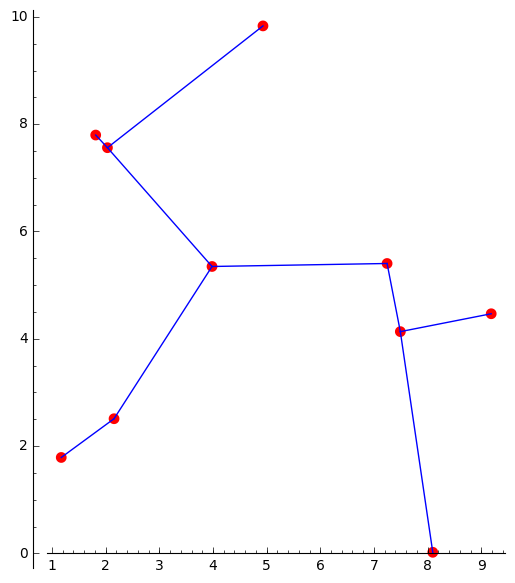
\includegraphics[scale=.6]{Figures/midterm_1.png} \\
      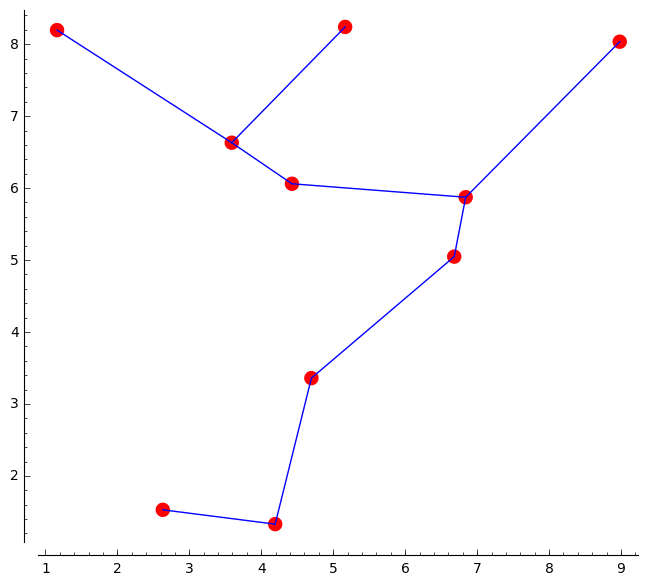
\includegraphics[scale=.5]{Figures/midterm_2.png}
    \end{center}

  \item % #4
    Consider the following problem. 
    Input is a connected graph $G=(V,E)$ and a cost function $c:E \rightarrow \RR$.
    Let $T$ be a spanning tree of $G$. The cost of $T$ is defined as the largest cost of an edge
    in $T$: 
    \[
      c(T) = \max*\{c(e): e \in E(T)\}.
    \]
    Problem is to find a minimum spanning tree with respect to $c$\\
    Do both a) and b):
    \begin{enumerate}
      \item[(a)]
        Formulate the problem using integer programming
      \item[(b)]
        Find an algorithm for solving this problem in polynomial time and prove its correctness.
    \end{enumerate}
\end{enumerate}
\end{document}
